\section{Speech Synthesis}
Di berbagai media, Anda mungkin pernah menyaksikan Stephen Hawking berbicara di depan mahasiswanya. Fisikawan yang terkenal dengan teori black hole-nya ini sudah tidak mampu lagi mengeluarkan suara dari lisannya, namun berkat teknologi speech synthesizer, dia masih bisa bercakap-cakap. Mesin speech synthesizer Hawking memang cukup kompleks. Alat ini tidak hanya memproduksi suara, tetapi juga menangkap input dari gerakan mata sang doktor. Demikian pula, misalnya, dengan aplikasi voice command yang banyak tertanam di smartphone mutakhir yang memadukan speech recognizer dengan speech synthesizer.

Aplikasi speech synthesizer yang paling sederhana sebenarnya ada pada setiap PC ber-OS Windows. Bila anda menekan tuts Winkey + U di keyboard, Windows akan mengaktifkan Utility Manager, yang di dalamnya terdapat aplikasi Microsoft Narrator. Aplikasi ini akan membaca setiap jendela yang anda aktifkan, termasuk tombol-tombol di dalamnya. Atau, mungkin anda pernah menginstal aplikasi microsoft reader di PC. Aplikasi yang diperuntukkan bagi file >LTT ini pun dilengkapi dengan kemampuan menerjemahkan teks menjadi suara (text to speech) yang merupakan contoh teknologi speech synthesizer.

\begin{figure}[H]
        \centerline{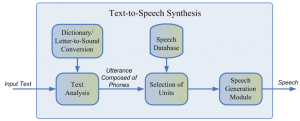
\includegraphics[scale=.75]{figures/speech}}
        \caption{Speech Synthesis}
		\label{speech}
\end{figure}

Speech synthesis adalah sebuah kemampuan bicara manusia yang dibuat oleh manusia (artificial). Sebuah sistem komputer digunakan untuk tujuan ini yang disebut sebagai speech synthesizer, dan dapat diimplementasikan ke dalam software atau hardware. Sebagai contoh sebuah sistem text-to-speech (TTS) yang dapat mengkonversikan teks dengan bahasa biasa menjadi suara.

Sebuah sistem komputer yang digunakan untuk tujuan ini disebut speech synthesizer, dan dapat diimplementasikan dalam perangkat lunak atau perangkat keras produk. Sebuah teks-to-speech (TTS) sistem mengkonversi teks bahasa normal menjadi berbicara; sistem lain membuat representasi linguistik simbolik seperti transkripsi fonetik ke dalam pidato, pidato disintesis dapat dibuat dengan menggabungkan potongan pidato direkam yang disimpan dalam database. Sistem berbeda dalam ukuran unit pidato disimpan, sebuah sistem yang menyimpan telepon atau diphones menyediakan berbagai keluaran terbesar, tapi mungkin kurang jelas.

Speech synthesis adalah transformasi dari teks ke arah suara (speech). Transformasi ini mengkonversi teks ke pemadu suara (speech synthesis) yang sebisa mungkin dibuat menyerupai suara nyata, disesuaikan dengan aturan – aturan pengucapan bahasa.TTS (text to speech) dimaksudkan untuk membaca teks elektronik dalam bentuk buku, dan juga untuk menyuarakan teks dengan menggunakan pemaduan suara. Sistem ini dapat digunakan sebagai sistem komunikasi, pada sistem informasi referral, dapat diterapkan untuk membantu orang-orang yang kehilangan kemampuan melihat dan membaca.

Synthesized speech dapat diciptakan dengan menggabungkan beberapa potongan-potongan dari pembicaraan/pidato yang sudah direkam dalam sebuah basis data. Kualitas dari sebuah speech synthesizer dilihat dari kemiripannya dengan suara manusia dan kemampuannya untuk bisa dipahami. Program TTS yang jelas dapat membantu orang dengan gangguan visual atau ketidakmampuan membaca, untuk mendengarkan pada pekerjaan yang tertulis dalam komputer. Banyak Sistem Operasi komputer yang telah dimasukkan speech synthesizer sejak tahun 1980-an.

Sebuah sistem text-to-speech (atau “mesin”) terdiri dari dua bagian: front-end dan back-end . Front-end memiliki dua tugas utama. Pertama, mengubah teks mentah berisi simbol seperti angka dan singkatan menjadi setara dengan kata-kata tertulis-out. Proses ini sering disebut normalisasi teks, pra-pengolahan, atau tokenization . Front-end kemudian memberikan transkripsi fonetik untuk setiap kata, dan membagi dan menandai teks ke unit prosodi , seperti frase , klausa , dan kalimat . Proses menetapkan transkripsi fonetik untuk kata-kata ini disebut teks-ke-fonem atau grafem konversi -untuk-fonem. Transkripsi fonetik dan informasi prosodi bersama-sama membentuk representasi linguistik simbolik yang output dengan front-end. Back-end-sering disebut sebagai synthesizer-maka mengubah representasi linguistik simbolik menjadi suara. Dalam sistem tertentu, bagian ini meliputi perhitungan dari target prosodi (kontur pitch, durasi fonem), yang kemudian dikenakan pada pidato output.

\subsection{Sejarah Speech Synthesis}
Upaya yang paling awal untuk menghasilkan lahirnya pemandu suara, pada abad XVIII. Terlepas dari kenyataan bahwa upaya pertama  adalah bentuk mesin mekanis, kita dapat mengatakan hari ini  bahwa synthesizer sudah berkualitas tinggi. Pada tahun 1779 di

St Petersburg, Rusia Profesor Kratzenshtein Kristen  fisiologis menjelaskan perbedaan antara lima vokal panjang  (/ A /, / e /, / i /, / o /, dan / u /) dan membuat alat untuk menghasilkan  mereka artifisial. Tahun 1791 di Wina, Wolfgang von Kempelen memperkenalkan nya “Akustik-Mekanik Mesin Speech”. Dalam  sekitar pertengahan 1800-an Charles Wheatstone dibangun terkenal  versi mesin berbicara von Kempelen’s.

Generasi dari sistem pemaduan suara ini dapat dibagi ke dalam 3 masa, yaitu:

\begin{enumerate}
\item Generasi pertama (1962-1977). Format sintesis dari fonem adalah teknologi dominan. Teknologi ini memanfaatkan aturan berdasarkan penguraian fonetik pada kalimat untuk kontur frekuensi forman. Beberapa sintesis masih miskin atau kurang dalam kejelasan dan kealamiannya.
\item Generasi kedua (1977-1992). Metode pemadu suara adalah diphone diwakilkan  dengan parameter LPC. Hal tersebut menunujukkan bahwa kejelasan yang baik pada pemadu suara dapat diperoleh dengan andal dari input teks dengan menggabungkan diphone yang sesuai dengan unit. Kejelasan meningkat selama sintesis forman, tetapi kealamian dari pemadu suara masih tetap rendah.
\item Generasi ketiga (1992-sekarang). Generasi ini ditandai dengan metode ‘ sintesis pemilihan unit’ yang diperkenalkan dan disempurnakan oelh Sagisaka di Labs ATR Kyoto. Hasil dari pemandu suara pada periode ini sangat mendekati human-generated speech pada bagian kejelasan dan kealamian.
\end{enumerate}

Teknologi pemadu suara modern melibatkan metode dan algoritma yang canggih dan rumit. alat pemadu suara  dari keluarga “Infovox” mungkin mejadi salah satu multi bahasa TTS yang paling dikenal saat ini. Versi komersial pertamanya, Infovox-SA 101, dikembangkan pada tahun 1982 di Institute Teknologi Royal, Swedia dan didasarkan pada sintesis forman.

AT \& T Bell Laboratories (Lucent Technologies) juga memiliki tradisi yang sangat panjang tentang pemandu suara (speech synthesis). TTS lengkap yang pertama didemostrasikan di Boston pada tahun 1972 dan diliris pada tahun 1973. Hal ini didasarkan pada model artikulatoris yang sikembangkan oleh Ceceil Coker (Klatt 1987). Pengembangan proses dari sistem penggabungan sintesis ini dimulai oleh Joseph Olive pada pertengahan tahun 1970-an (Bell Labs 1997). Sistem ini sekarang sudah tersedia untuk bahasa Inggris, Perancis, Spanyol, Italia, Jerman, Rusia, Rumania, Cina, dan Jepang (Mcbius et al 1996).

\begin{figure}[H]
        \centerline{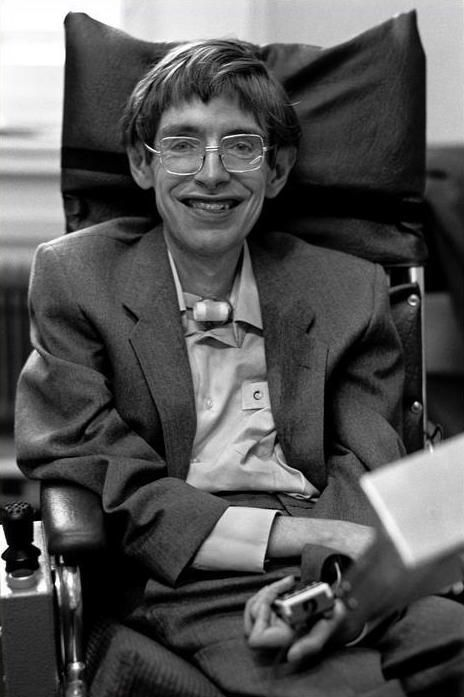
\includegraphics[scale=.45]{figures/stephan}}
        \caption{Stephen Hawking adalah salah satu orang paling terkenal yang menggunakan sintesis ucapan untuk berkomunikasi}
		\label{stephan}
\end{figure}

\subsection{Perangkat Speech Synthesis}
Pidato sistem sintesis berbasis komputer pertama diciptakan pada akhir 1950-an. Pertama umum Inggris sistem text-to-speech dikembangkan oleh Noriko Umeda et al. Pada tahun 1968 di Laboratorium Elektroteknik, Jepang. Pada tahun 1961, fisikawan John Larry Kelly, Jr dan Louis rekan Gerstman menggunakan IBM 704 komputer untuk mensintesis pidato, acara yang paling menonjol dalam sejarah Bell Labs . Kelly perekam suara synthesizer ( vocoder ) ulang lagu ” Daisy Bell “, dengan iringan musik dari Max Mathews .Kebetulan, Arthur C. Clarke mengunjungi teman dan kolega John Pierce di fasilitas Bell Labs Murray Hill. Clarke begitu terkesan oleh demonstrasi bahwa ia digunakan dalam adegan klimaks dari skenario-Nya untuk novel nya 2001: A Space Odyssey, di mana HAL 9000 komputer menyanyikan lagu yang sama seperti yang sedang ditidurkan oleh astronot Dave Bowman. Meskipun keberhasilan pidato sintesis murni elektronik, penelitian masih terus dilakukan ke synthesizer pidato mekanis.

Handheld elektronik menampilkan sintesis pidato mulai muncul pada 1970-an. Salah satu yang pertama adalah Telesensory Systems Inc(TSI) Pidato + kalkulator portabel untuk orang buta pada tahun 1976. Perangkat lain yang diproduksi terutama untuk tujuan pendidikan, seperti Bicara \& Eja , yang diproduksi oleh Texas Instruments pada tahun 1978. Fidelity merilis versi berbicara komputer catur elektronik pada tahun 1979. Yang pertama video game yang memiliki fitur sintesis pidato adalah 1.980 shoot ’em up arcade game , Stratovox , dari Sun Electronics. Contoh lain awal adalah versi arcade dari Berzerk , dirilis pada tahun yang sama.Pertama multi-player permainan elektronik menggunakan sintesis suara adalah Milton dari Milton Bradley Company , yang memproduksi perangkat di tahun 1980.

\subsection{Teknologi Speech Synthesis}
Yang paling penting dalam kualitas sistem speech synthesis adalah kealamian dan kejelasannya. Kealamaian menjelaskan bagaimana dekatnya suara output dengan suara manusia, sementara kejelasan adalah dengan kemudahan di mana output tersebut dapat dipahami. Speech synthesizer yang ideal adalah yang alami dan jelas. Sistem speech synthesis biasanya mencoba untuk memaksimalkan kedua karakteristik.

Kualitas terpenting dari sebuah aplikasi speech synthesizer adalah seberapa alami dan inteligibel output yang dihasilkannya. Alami, artinya seberapa dekat suara yang dihasilkan aplikasi speech synthesizer dengan suara manusia. Sedangkan inteligibel adalah seberapa mudah output tersebut dipahami oleh manusia. Semua aplikasi speech synthesizer berusaha untuk menghasilkan output yang alami dan inteligibel sekaligus.

Sampai saat ini, ada banyak teknologi untuk meng-generate gelombang suara sintetis ini. Dua teknologi yang paling banyak digunakan adalah concatenative synthesis dan formant synthesis. Keduanya memiliki keunggulan dan kekurangan sendiri-sendiri.

Teknologi pertama, concatenative synthesis, berbasis pada rangkaian (atau merangkai bersama) segmen-segmen dari suara yang direkam. Umumnya, teknologi ini menghasilkan suara sintesis yang terdengar paling alami.Namun, perbedaan antara suara alami yang direkam dengan segmentasi gelombang bunyi kadang menghasilkan suara yang menggangu. Mirip seperti suara pemberitahuan nomor antrean di bank atau suara call center operator ponsel yang menyebutkan sisa pulsa dan masa berlaku kartu ponsel anda.

Teknologi kedua, formant synthesis, tidak menggunakan sampel suara manusia melainkan membuat suara sintesi menggunakan model akustik. Parameter-parameter seperti frekuensi dasar, alunan suara, dan tingkat kebisingan bervariasi dari waktu ke waktu untuk menciptakan gelombang suara buatan.

Kebanyakan aplikasi berbasis teknologi ini menghasilkan suara buatan (tidak alami) seperti suara robot. Melihat keterbatasan kedua teknologi ini dalam menghasilkan suara buatan, seperti kita harus sabar menunggu pengembangannya lebih lanjut dalam beberapa tahun atau dekade ke depan.

Kualitas yang paling penting dari sebuah sistem sintesis pidato kewajaran dan dimengerti. kealamian menjelaskan seberapa dekat output terdengar seperti suara manusia, sementara kejelasan adalah kemudahan yang output dipahami. Speech synthesizer yang ideal adalah baik alam dan dimengerti. Sistem sintesis pidato biasanya mencoba untuk memaksimalkan kedua karakteristik.

Dua teknologi utama dalam pembuatan gelombang suara synthetic speech adalah Concatenative Synthesis dan Formant Synthesis. Setiap teknologi mempunyai kekuatan dan kelemahannya, dan penggunaan yang ditujukan dari sistem synthesis akan menentukkan pendekatan mana yang digunakan.

\begin{enumerate}
\item Concatenative Synthesis
Concantenative synthesis didasarkan dengan penggabungan dari segmen-segmen dari pembicaraan yang sudah direkam. Secara umum, concatenative synthesis memproduksi synthesized speech dengan suara yang paling alami. Tetapi, perbedaan antara variasi alami dalam pembicaraaan dan sifat dari teknik otomasi untuk pensegmentasian gelombang suara terkadang menghasilkan kesalahan suara dalam output. Namun, perbedaan antara variasi alami dalam pidato dan sifat teknik otomatis untuk membagi bentuk gelombang kadang-kadang menyebabkan gangguan terdengar pada output. Ada tiga sub-jenis utama dari sintesis concatenative.
\begin{enumerate}
\item Sintesis Pemilihan unit
Sintesis Pemilihan unit menggunakan besar database pidato direkam. Selama pembuatan database, setiap ucapan tercatat tersegmentasi ke dalam beberapa atau semua hal berikut: individu telepon , diphones , setengah-telepon, suku kata , morfem , kata , frase , dan kalimat . Biasanya, pembagian ke dalam segmen dilakukan dengan menggunakan dimodifikasi khusus recognizer pidato disetel ke “keselarasan dipaksa” mode dengan beberapa koreksi manual setelah itu, dengan menggunakan representasi visual seperti yang gelombang dan spektogram .  Sebuah indeks unit dalam database pidato kemudian dibuat berdasarkan segmentasi dan parameter akustik seperti frekuensi dasar (lapangan ), durasi, posisi dalam suku kata, dan telepon tetangga. Pada waktu berjalan , target ucapan yang diinginkan dibuat dengan menentukan rantai terbaik unit calon dari database (pemilihan unit). Proses ini biasanya dicapai dengan menggunakan khusus tertimbang pohon keputusan.

Pemilihan unit menyediakan kealamian terbesar, karena hanya berlaku sedikit pemrosesan sinyal digital (DSP) untuk pidato direkam. DSP sering membuat pidato yang direkam terdengar kurang alami, meskipun beberapa sistem menggunakan sejumlah kecil pengolahan sinyal pada titik Rangkaian untuk menghaluskan bentuk gelombang. Output dari yang terbaik unit-seleksi sistem sering dibedakan dari suara manusia nyata, terutama dalam konteks dimana sistem TTS telah disetel. Namun, kealamian maksimum biasanya membutuhkan unit-pilihan database pidato menjadi sangat besar, dalam beberapa sistem mulai ke gigabyte data dicatat, mewakili puluhan jam berbicara.  Juga, pilihan algoritma Unit telah dikenal untuk memilih segmen dari Tempat yang menghasilkan kurang dari sintesis ideal (misalnya kata-kata kecil menjadi tidak jelas) bahkan ketika pilihan yang lebih baik ada dalam database. Baru-baru ini, peneliti telah mengusulkan berbagai metode otomatis untuk mendeteksi segmen alami di unit-pilihan sistem sintesis pidato.
\item Sintesis diphone
Sintesis diphone menggunakan database pidato minimal berisi semua diphones (suara-to-suara transisi) yang terjadi dalam suatu bahasa. Jumlah diphones tergantung pada fonotaktik bahasa: misalnya, Spanyol memiliki sekitar 800 diphones, dan Jerman sekitar 2500. Dalam sintesis diphone, hanya satu contoh dari setiap diphone terkandung dalam database pidato. Pada saat runtime, target prosodi kalimat ditumpangkan pada unit-unit minimal dengan cara pemrosesan sinyal digital teknik seperti linear predictive coding ,PSOLA atau MBROLA. Diphone sintesis menderita gangguan sonik sintesis concatenative dan robot-terdengar sifat sintesis forman, dan memiliki beberapa keuntungan baik pendekatan lain dari ukuran kecil. Dengan demikian, penggunaannya dalam aplikasi komersial menurun, meskipun terus digunakan dalam penelitian karena ada beberapa implementasi perangkat lunak tersedia secara bebas.
\item Domain-spesifik sintesis
Domain-spesifik sintesis concatenates direkam sebelumnya kata dan frase untuk menciptakan ucapan-ucapan yang lengkap. Hal ini digunakan dalam aplikasi di mana berbagai teks output sistem akan terbatas pada domain tertentu, seperti jadwal angkutan pengumuman atau laporan cuaca.  Teknologi ini sangat sederhana untuk menerapkan, dan telah digunakan secara komersial untuk waktu yang lama , dalam perangkat seperti berbicara jam dan kalkulator. Tingkat kealamian sistem ini bisa sangat tinggi karena berbagai jenis kalimat terbatas, dan mereka cocok dengan prosodi dan intonasi dari rekaman asli.

Karena sistem ini dibatasi oleh kata-kata dan frasa dalam database mereka, mereka tidak tujuan umum dan hanya dapat mensintesis kombinasi kata dan frase yang mereka telah terprogram. Campuran kata-kata dalam bahasa alami diucapkan namun masih dapat menyebabkan masalah kecuali banyak variasi diperhitungkan. Misalnya, dalam non-rhotic dialek dari bahasa Inggris “r” dalam kata-kata seperti “jelas” biasanya hanya diucapkan ketika kata berikut memiliki vokal sebagai huruf pertama (misalnya”membersihkan” direalisasikan sebagai  ). Demikian juga di Perancis , banyak konsonan akhir menjadi tidak lagi diam jika diikuti oleh sebuah kata yang dimulai dengan vokal, efek yang disebut penghubung . Ini pergantian tidak bisa direproduksi oleh sistem kata-Rangkaian sederhana, yang akan membutuhkan kompleksitas tambahan untuk konteks-sensitif .
\end{enumerate}
\item Formant Synthesis
Formant synthesis tidak menggunakan pembicaraan manusia sebagai sample pada runtime. Daripada itu, synthesized speech yang dihasilkan dibuat dengan additive synthesis dan sebuah model akustik (physical modelling synthesis).

Parameter seperti frekuensi dasar, penyuaraan, dan tingkat kebisingan di variasikan dari waktu ke waktu untuk menciptakan gelombang buatan (artificial) dari sebuah pembicaraan. Banyak sistem yang berdasarkan formant synthesis menciptakan pembicaraan yang seperti robot yang tidak mungkin dapat dikenal sebagai suara manusia. Tetapi, kealamian maksimum bukan selalu tujuan dari sebuah sistem speech synthesis, dan sistem formant synthesis mempunyai keuntungan dari sistem concatenative. Pembicaraan yang di-formant synthesis-kan dapat menjadi sangat jelas, bahkan dalam kecepatan yang tinggi, sehingga menghindari kesalahan suara yang sering dialami sistem concatenative.

Formant synthesis biasanya program yang lebih kecil dari concatenative sistem karena ia tidak menggunakan basis data dari sampel-sampel pembicaraan. Oleh karena itu formant synthesis dapat ditanamkan dalam sistem yang mempunyai memory dan microprosesor yang terbatas. Karena sistem yang berdasarkan formant mempunyai kendali penuh dari sluruh aspek dari hasil pembicaraan, variasi yang luas dari prosodi dan intonasi dapat dihasilkan, menyampaikan tidak hanya pertanyaan dan pernyataan tetapi juga emosi dan nada suara.

Formant sintesis tidak menggunakan sampel suara manusia pada saat runtime. Sebaliknya, keluaran suara yang disintesis dibuat menggunakan aditif sintesis dan model akustik (sintesis pemodelan fisik ). Parameter seperti frekuensi dasar , menyuarakan , dan kebisingan tingkat yang bervariasi dari waktu ke waktu untuk membuat gelombang pidato buatan. Metode ini kadang-kadang disebut aturan berbasis sintesis; Namun, banyak sistem concatenative juga memiliki aturan berbasis komponen. Banyak sistem yang didasarkan pada teknologi sintesis forman menghasilkan buatan, robot yang terdengar pidato yang tidak akan pernah salah untuk pidato manusia. Namun, kealamian maksimum tidak selalu tujuan sistem sintesis pidato, dan sistem sintesis forman memiliki keunggulan dibandingkan sistem concatenative. Pidato forman-disintesis dapat diandalkan dimengerti, bahkan pada kecepatan yang sangat tinggi, menghindari Glitches akustik yang biasanya wabah sistem concatenative. Kecepatan tinggi disintesis pidato digunakan oleh tunanetra untuk navigasi cepat komputer menggunakan pembaca layar . Synthesizer forman adalah program biasanya lebih kecil dibandingkan dengan sistem concatenative karena mereka tidak memiliki database contoh pidato. Karena itu mereka dapat digunakan dalam embedded system , di mana memori dan mikroprosesor daya terutama terbatas. Karena sistem berbasis forman memiliki kontrol penuh dari semua aspek pidato output, berbagai prosodies dan intonasi dapat menjadi output, tidak hanya menyampaikan pertanyaan dan pernyataan, tetapi berbagai emosi dan nada suara.

Contoh non-real-time tapi sangat akurat kontrol intonasi dalam sintesis forman meliputi pekerjaan yang dilakukan pada akhir tahun 1970 untuk Texas Instruments mainan Bicara \& Eja , dan pada awal tahun 1980 Sega arcade mesin dan dalam banyak Atari, Inc. game arcade menggunakan TMS5220 LPC Chips . Menciptakan intonasi yang tepat untuk proyek ini adalah telaten, dan hasilnya masih harus dicocokkan dengan real-time text-to-speech interface.
\item Sintesis artikulatoris
Sintesis artikulatoris mengacu pada teknik komputasi untuk sintesis pidato berdasarkan model manusia saluran vokal dan artikulasi proses yang terjadi di sana. Synthesizer artikulatoris pertama teratur digunakan untuk percobaan laboratorium dikembangkan di Haskins Laboratories di pertengahan 1970-an oleh Philip Rubin, Tom Baer, dan Paul Mermelstein. Synthesizer ini, yang dikenal sebagai ASY, didasarkan pada model saluran vokal dikembangkan di Bell Laboratories pada tahun 1960 dan 1970-an oleh Paul Mermelstein, Cecil Coker, dan rekan.

Sampai saat ini, model sintesis artikulatoris belum dimasukkan ke dalam sistem sintesis pidato komersial. Sebuah pengecualian adalah NeXT sistem berbasis awalnya dikembangkan dan dipasarkan oleh Trillium Suara Research, sebuah perusahaan spin-off dari University of Calgary , di mana banyak riset asli dilakukan. Setelah runtuhnya berbagai inkarnasi NeXT (dimulai oleh Steve Jobs pada akhir tahun 1980 dan bergabung dengan Apple Computer pada tahun 1997), perangkat lunak TRILLIUM diterbitkan di bawah GNU General Public License , dengan bekerja terus sebagai gnuspeech . Sistem, pertama kali dipasarkan pada tahun 1994, memberikan penuh text-to-speech konversi berbasis artikulatoris menggunakan Waveguide atau transmisi-line analog dari saluran mulut dan hidung manusia dikendalikan oleh Carré ini “model daerah khas”.
\item Sintesis berbasis HMM
Sintesis berbasis HMM  adalah metode sintesis berdasarkan model Markov tersembunyi , juga disebut statistik Parametrik Sintesis. Dalam sistem ini, spektrum frekuensi ( vokal ),frekuensi dasar (sumber vokal), dan durasi ( prosodi ) berbicara dimodelkan secara bersamaan oleh HMMs. Pidato bentuk gelombang yang dihasilkan dari HMMs sendiri berdasarkan maksimum kriteria.
\item Sintesis Sinewave
Sintesis sinewave adalah teknik untuk sintesis pidato dengan mengganti forman (band utama energi) dengan peluit nada murni.

Ada beberapa masalah yang terdapat pada pemaduan suara, yaitu:
\begin{enumerate}
\item User sangat sensitif terhadap variasi dan informasi suara. Oleh sebab itu, mereka tidak dapat memberikan toleransi atas ketidaksempurnaan pemadu suara.
\item Output dalam bentuk suara tidak dapat diulang atau dicari dengan mudah.
\item Meningkatkan keberisikan pada lingkungan kantor atau jika menggunakan handphone, maka akan meningkatkan biaya pengeluaran.
\end{enumerate}
\end{enumerate}
